\clearpage
\VerdierPhysicalPageAnchor{0102}%
\begingroup
\small
\setlength{\abovedisplayskip}{3pt plus 2pt minus 2pt}%
\setlength{\belowdisplayskip}{3pt plus 2pt minus 2pt}%
\setlength{\jot}{2pt}%
\VerdierSemanticAnchor{ch1-3-4-1-proof}
由 (3.3.1)，总可以假定所给三角具有如下形式：

\VerdierSemanticAnchor{ch1-3-4-1-cone-model}
\[
  X\xrightarrow{\dot f}Y\xrightarrow{\dot p(f)}c(f)
  \xrightarrow{\dot q(f)}X[1]
\]
其中 $f\colon X\longrightarrow Y$ 是 $\operatorname{comp}(C)$ 中的态射。
只需证明三角

\VerdierSemanticAnchor{ch1-3-4-1-goal-triangle}
\[
  (\iota_1X)[-1]\xrightarrow{\iota_1\dot q(f)}\iota_1c(f)
  \xrightarrow{\iota_1\dot p(f)}\iota_1Y
  \xrightarrow{-(\iota_1\dot f)}\iota_1X
\]
是特异三角（$\iota_1f$ 是态射 $f$ 在
$\iota_1\colon\operatorname{comp}(C)^{\circ}\longrightarrow
\operatorname{comp}(C^{\circ})$ 下的像）。由 $\iota_1$ 的定义 (2.4.1) 以及
映射锥函子的定义 (3.1.2)，立即可知复形 $\iota_1c(f)$ 的分量和微分为

\VerdierSemanticAnchor{ch1-3-4-1-components}
\[
  \iota_1c(f)^i=(\iota_1X)^{i-1}\oplus(\iota_1Y)^i,
\]
\VerdierSemanticAnchor{ch1-3-4-1-1}
\begin{equation}
  d_{\iota_1c(f)}^i=
  \begin{pmatrix}
    -d_{\iota_1X}^{i-1} & (\iota_1f)^i\\
    0 & d_{\iota_1Y}^{i}
  \end{pmatrix}.
  \tag{3.4.1.1}
\end{equation}
\VerdierSemanticAnchor{ch1-3-4-1-cone-identity}
因此
\[
  \iota_1c(f)=c(-\iota_1f)[-1],
\]
并且可验证下图交换：

\VerdierSemanticAnchor{ch1-3-4-1-comparison}
\begin{center}
  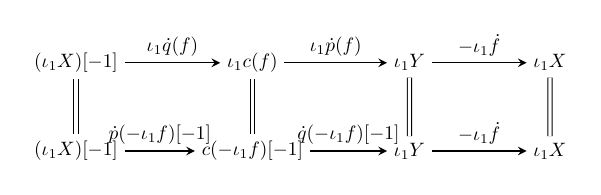
\begin{tikzpicture}[>=stealth,scale=0.70,every node/.style={transform shape}]
    \node (x1) at (0,1.60) {$(\iota_1X)[-1]$};
    \node (c1) at (3.20,1.60) {$\iota_1c(f)$};
    \node (y1) at (6.05,1.60) {$\iota_1Y$};
    \node (z1) at (8.60,1.60) {$\iota_1X$};
    \node (x2) at (0,0) {$(\iota_1X)[-1]$};
    \node (c2) at (3.20,0) {$c(-\iota_1f)[-1]$};
    \node (y2) at (6.05,0) {$\iota_1Y$};
    \node (z2) at (8.60,0) {$\iota_1X$};
    \draw[->] (x1) -- node[above] {$\iota_1\dot q(f)$} (c1);
    \draw[->] (c1) -- node[above] {$\iota_1\dot p(f)$} (y1);
    \draw[->] (y1) -- node[above] {$-\iota_1\dot f$} (z1);
    \draw[->] (x2) -- node[above] {$\dot p(-\iota_1f)[-1]$} (c2);
    \draw[->] (c2) -- node[above] {$\dot q(-\iota_1f)[-1]$} (y2);
    \draw[->] (y2) -- node[above] {$-\iota_1\dot f$} (z2);
    \draw[double,double distance=1.1pt] (x1) -- (x2);
    \draw[double,double distance=1.1pt] (c1) -- (c2);
    \draw[double,double distance=1.1pt] (y1) -- (y2);
    \draw[double,double distance=1.1pt] (z1) -- (z2);
  \end{tikzpicture}
\end{center}
\VerdierSemanticAnchor{ch1-3-4-1-proof-complete}
于是应用 (3.3.3) 即完成证明。

\VerdierSemanticAnchor{ch1-3-4-2}
\noindent\textbf{3.4.2.}\quad
\VerdierSemanticAnchor{ch1-3-4-2-multiadditive-functor}
设 $F\colon\prod_{i\in[n]}C_i\longrightarrow C$ 为多加法函子。为具体起见，
假定 $C$ 中可数乘积可表示。设
\[
  K_{\Pi}F\colon\prod_{i\in[n]}K(C_i)\longrightarrow K(C)
\]
\VerdierSemanticAnchor{ch1-3-4-2-homotopy-extension}
为 $F$ 在复形同伦范畴上的 $\Pi$-扩张，并设

\VerdierSemanticAnchor{ch1-3-4-2-shift-isomorphisms}
\[
  p_i\colon K_{\Pi}F(X_1,\ldots,X_i[1],\ldots,X_n)
  \longrightarrow K_{\Pi}F(X_1,\ldots,X_i,\ldots,X_n)[1]
\]
为典范函子同构。
\endgroup
